% Birlesik rapor. Derleme: tectonic -X compile birlesik_rapor.tex  (rapor\ klasorunde; fontlar ../fontlar)
\documentclass[10.5pt,a4paper]{article}
% Ortak onbilgi: uc "Study of Simulation Tools" raporu icin. Derleme: tectonic -X compile <dosya>.tex (rapor\ klasorunde)
\usepackage{fontspec}
\setmainfont{georgia}[Path=../fontlar/,Extension=.ttf,BoldFont=georgiab,ItalicFont=georgiai,BoldItalicFont=georgiaz]
\setsansfont{arial}[Path=../fontlar/,Extension=.ttf,BoldFont=arialbd,ItalicFont=ariali,BoldItalicFont=arialbi]
\setmonofont{consola}[Path=../fontlar/,Extension=.ttf,BoldFont=consolab,ItalicFont=consolai,BoldItalicFont=consolaz,Scale=0.86]
\usepackage[a4paper,left=2.2cm,right=2.2cm,top=1.9cm,bottom=1.8cm]{geometry}
\usepackage{xcolor,graphicx,titlesec,enumitem,amsmath,booktabs,xltabular,listings,fancyhdr,caption}
\emergencystretch=3em
\definecolor{ink}{HTML}{1F2937}\definecolor{acc}{HTML}{1D4ED8}\definecolor{muted}{HTML}{6B7280}\definecolor{codebg}{HTML}{F3F4F6}
\color{ink}
\titleformat{\section}{\sffamily\bfseries\large\color{acc}}{}{0pt}{}
\titlespacing*{\section}{0pt}{9pt}{3pt}
\titleformat{\subsection}{\sffamily\bfseries\normalsize}{}{0pt}{}
\titlespacing*{\subsection}{0pt}{6pt}{2pt}
\setlength{\parindent}{0pt}\setlength{\parskip}{4pt plus 1pt}
\setlist{itemsep=1pt,topsep=2pt,parsep=0pt}
\pagestyle{fancy}\fancyhf{}\renewcommand{\headrulewidth}{0.3pt}
\fancyhead[L]{\sffamily\footnotesize\color{muted} EHB415 \textbullet\ Study of Simulation Tools}
\fancyfoot[C]{\sffamily\footnotesize\color{muted}\thepage}
\captionsetup{font={sf,footnotesize},labelfont=bf,labelsep=period,skip=2pt}
\lstset{basicstyle=\ttfamily\footnotesize,backgroundcolor=\color{codebg},frame=single,rulecolor=\color{codebg!70!black},
  breaklines=true,columns=fullflexible,keepspaces=true,showstringspaces=false,aboveskip=4pt,belowskip=6pt,
  literate={ğ}{g}1 {ş}{s}1 {ı}{i}1 {ü}{u}1 {ö}{o}1 {ç}{c}1}
\newcommand{\baslik}[2]{%
  {\sffamily\color{muted}\small EHB415 Dönem Projesi \textbullet\ 2026--2027 Güz\par}
  {\sffamily\bfseries\Large Study of Simulation Tools: #1\par}
  {\sffamily\small #2\par}
  \vspace{-2pt}{\color{acc!40}\rule{\textwidth}{0.8pt}}\par}
\IfFileExists{isimler.tex}{\input{isimler}}{\newcommand{\taha}{[Ad Soyad -- No]}\newcommand{\aziz}{[Ad Soyad -- No]}\newcommand{\fatih}{[Ad Soyad -- No]}\newcommand{\nihat}{[Ad Soyad -- No]}}

\titleformat{\subsubsection}{\sffamily\bfseries\small\color{ink}}{}{0pt}{}
\titlespacing*{\subsubsection}{0pt}{5pt}{2pt}
\begin{document}
\begin{center}
{\sffamily\color{muted}\small EHB415 Dönem Projesi \textbullet\ 2026--2027 Güz \textbullet\ Study of Simulation Tools\par}
\vspace{6pt}
{\sffamily\bfseries\LARGE Integrating Sensing Capabilities into 5G Networks:\\ An ISAC-Oriented Study\par}
\vspace{8pt}
{\sffamily\small \taha \quad \aziz\par \fatih \quad \nihat\par}
\end{center}
\vspace{-4pt}{\color{acc!40}\rule{\textwidth}{0.8pt}}

\section*{1. Projenin amacı ve bu raporun kapsamı}
Entegre algılama ve haberleşme (ISAC), kablosuz altyapının hem veri taşıdığı hem de çevreyi algıladığı yeni bir yaklaşımdır. 5G-Advanced ve 6G'de algılama yeteneği eklemek; kaynak ayırma, işlem yükü ve haberleşme başarımı üzerindeki etki gibi soruları gündeme getirir. Projemiz, ISAC işlevlerinin açık kaynaklı bir 5G ağ mimarisine (OCUDU) nasıl eklenebileceğini inceler ve bunların etkisini benzetim araçlarıyla değerlendirir. Hedefler: (i) 3GPP ISAC çalışmalarını gözden geçirmek, (ii) seçilen işlevlerin OCUDU içinde veya yanında nasıl uygulanabileceğini araştırmak, (iii) benzetime dayalı bir değerlendirme çerçevesi kurmak, (iv) algılama ile haberleşme başarımı arasındaki ödünleşimi (trade-off) değerlendirmek.

Bu rapor, projede kullanacağımız üç aracın \textbf{doğru kurulduğunu ve çalıştığını} gösterir: \textbf{ns-3 + 5G-LENA}, \textbf{OCUDU} ve \textbf{Sionna}. Araçlar tek bir soruyu üç yönden ölçer: \emph{algılamaya ne kadar kaynak ayırırsak algılama ne kazanır, haberleşme ne kaybeder?} Ortak eksen, algılamaya giden kaynak payıdır ($\alpha$).

\begin{center}\sffamily\small
\begin{tabular}{@{}p{2.6cm}p{3.3cm}p{3.3cm}p{4.2cm}@{}}
\toprule
\textbf{Araç} & \textbf{Projedeki rolü} & \textbf{Sürüm / ortam} & \textbf{Doğrulama} \\
\midrule
ns-3 + 5G-LENA & Haberleşme maliyeti (ağ düzeyi) & ns-3.48, nr v5.1; WSL2 Ubuntu 24.04 & \texttt{cttc-nr-demo} çalıştı, kendi programımız elle hesapla tuttu \\
OCUDU & Haberleşme maliyeti (gerçek gNB kodu) & 26.10.0; WSL2 Ubuntu 24.04, Clang 18 & \texttt{testmode}: DL $\approx$59 Mbps, UL 77,3 Mbps, 1000 blok/s \\
Sionna / Sionna RT & Algılama kazancı (kanal ve radar) & 1.2.2; Ubuntu 22.04 ve Windows 11 & Radar testi hata çözünürlük içinde; ışın izleme 12 yol \\
\bottomrule
\end{tabular}
\end{center}

\section*{2. Bölüm A: ns-3 ve 5G-LENA}
{\sffamily\small Hazırlayan: \aziz\par}

\subsection*{Projedeki yeri ve araç seçimi}
Projemiz, 5G baz istasyonunun algılama (sensing) için ayırdığı kaynak payının ($\alpha$) haberleşmeye maliyetini ölçmeyi amaçlıyor. ns-3 bu maliyeti \textbf{çok kullanıcılı bir ağda}, yani kullanıcı sayısı arttıkça throughput ve gecikmenin nasıl değiştiğini ölçmek için kullanılacak. ns-3, açık kaynaklı bir ağ simülatörüdür. 5G NR için CTTC'nin geliştirdiği \textbf{5G-LENA} (\texttt{nr} modülü) ns-3'e eklenerek kullanılır. Seçim nedenleri: 5G NR'nin MAC düzeyindeki zamanlayıcılarını (scheduler) içermesi, hazır 5G örnekleri sunması ve akış düzeyinde throughput ile gecikme ölçebilmesi. 5G-LENA her sürüm için belirli bir ns-3 sürümünü önerir; biz \textbf{ns-3.48 + 5G-LENA v5.1} çiftini kullandık.

\subsection*{Kurulum}
\begin{center}\sffamily\small
\begin{tabular}{@{}ll@{}}
\toprule
Ortam & Windows 11 üzerinde WSL2, Ubuntu 24.04.5 LTS \\
Derleyici ve araçlar & g++ 13.3.0, CMake 3.28.3, Ninja \\
Simülatör & ns-3.48 (\texttt{\textasciitilde/ehb415/ns-3-dev}) \\
5G modülü & 5G-LENA v5.1 (\texttt{contrib/nr}) \\
Derleme profili & optimized (\texttt{-d optimized}), 1876 hedef \\
Süre ve disk & yaklaşık 18 dakika (\texttt{-j6}), yaklaşık 0,5 GB \\
\bottomrule
\end{tabular}
\end{center}
Kurulum komutları (Ubuntu terminalinde; ayrıntı: projedeki \texttt{kurulum/04-ns3-5g-lena.md}):
\begin{lstlisting}
sudo apt-get update
sudo apt-get install -y build-essential g++ python3 python3-venv python3-pip cmake \
    ninja-build git ccache pkg-config libc6-dev sqlite3 libsqlite3-dev libeigen3-dev
mkdir -p ~/ehb415 && cd ~/ehb415
git clone --depth 1 --branch ns-3.48 https://gitlab.com/nsnam/ns-3-dev.git
git clone --depth 1 --branch v5.1 https://gitlab.com/cttc-lena/nr.git ns-3-dev/contrib/nr
cd ns-3-dev
./ns3 configure --enable-examples -d optimized -G Ninja
./ns3 build -j6
\end{lstlisting}
5G-LENA klasörünün adı \texttt{nr} olmalı ve \texttt{contrib/} altında durmalı.

\subsection*{Karşılaşılan sorunlar ve çözümleri}
\begingroup\sffamily\small
\begin{xltabular}{\textwidth}{@{}p{4.3cm}X@{}}
\toprule
\textbf{Sorun} & \textbf{Neden ve çözüm} \\
\midrule
\texttt{WSL2 is unable to start since virtualization is not enabled} & WSL kurulduktan sonra gerçek yeniden başlatma yapılmamıştı. Windows'ta Hızlı Başlatma açıkken Kapat--aç yetmiyor. \textbf{Başlat $\rightarrow$ Güç $\rightarrow$ Yeniden başlat} ile çözüldü. \\
Derleme sırasında \texttt{Killed} & Bellek yetmiyor. \texttt{.wslconfig} dosyasında \texttt{memory=10GB} ayarlandı, \texttt{-j6} yerine gerekirse \texttt{-j4} veya \texttt{-j2} kullanılır. \\
PowerShell'den \texttt{wsl -- bash -c '...'} ile karmaşık komutlar bozuluyor & Tırnak ve \texttt{\$}, \texttt{|} gibi karakterler PowerShell ile bash arasında karışıyor. Komutlar bir \texttt{.sh} dosyasına yazılıp \texttt{wsl -- bash dosya.sh} ile çalıştırıldı. \\
Simülasyon çıktısında \texttt{NS\_LOG} mesajları yok & ``optimized'' profilde günlük (log) çıktıları derlemeden çıkarılıyor. Sonuçlar akış izleyicisi (FlowMonitor) ve \texttt{trace} geri çağırmalarından okunuyor. Günlük gerekirse \texttt{-d debug} ile yeniden yapılandırılır. \\
Başka ns-3 sürümüyle derleme denemesi & 5G-LENA v5.1, ns-3.48 için tasarlandı; ns-3.49 gibi sürümlerle denenmemeli. \\
\bottomrule
\end{xltabular}
\endgroup

\subsection*{Örnek çalıştırma}
\subsubsection*{5G-LENA'nın hazır örneği: \texttt{cttc-nr-demo}}
Kurulumun doğru olduğunu görmek için 5G-LENA örneğini 2 kullanıcı ve 1 saniye simülasyonla çalıştırdım.
\begin{figure}[h!]
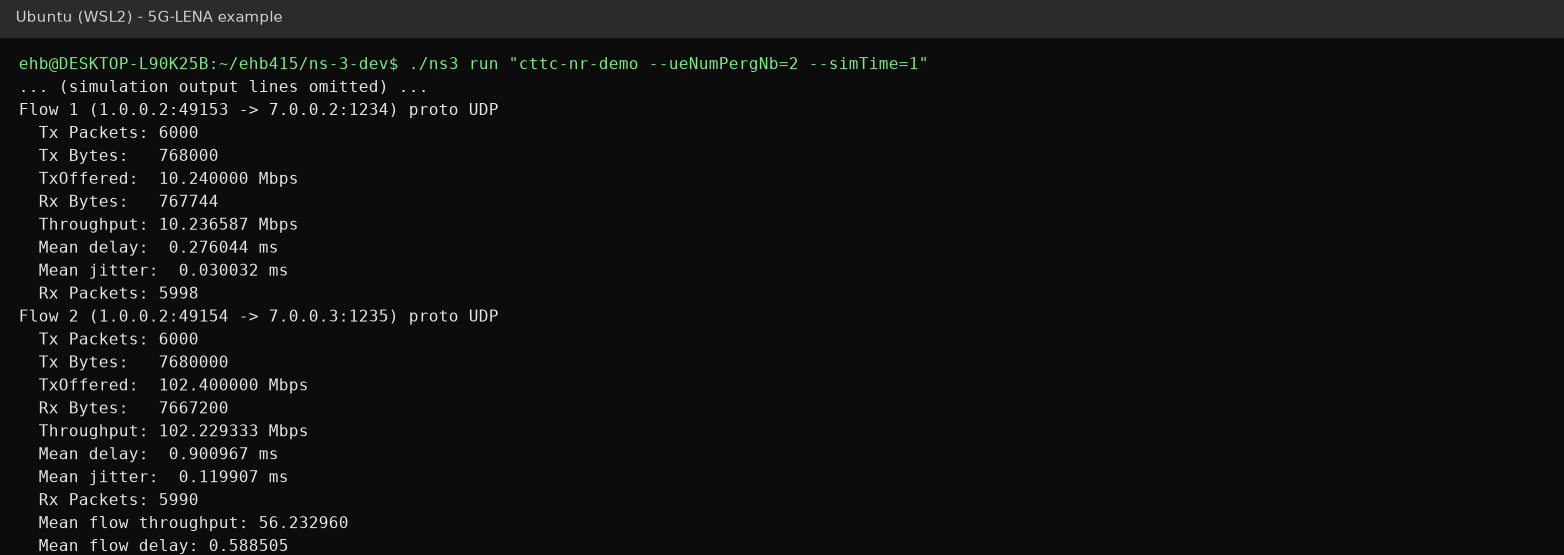
\includegraphics[width=\textwidth]{img/ns3_rapor_demo.png}
\caption{\texttt{cttc-nr-demo} çıktısının akış sonuçları (WSL2 Ubuntu terminali).}
\end{figure}

\begin{center}\sffamily\small
\begin{tabular}{@{}lrrrr@{}}
\toprule
 & Gönderilen & Alınan & Gecikme & Paket kaybı \\
\midrule
Akış 1 & 10,24 Mbps & 10,24 Mbps & 0,28 ms & \%0,03 \\
Akış 2 & 102,40 Mbps & 102,23 Mbps & 0,90 ms & \%0,17 \\
Ortalama (\texttt{Mean flow}) & & 56,23 Mbps & 0,59 ms & \\
\bottomrule
\end{tabular}
\end{center}
Alınan veri gönderilene çok yakın ve gecikme 1\,ms altında. Yük kapasitenin altında olduğu için bu beklenen bir sonuç.

\subsubsection*{Kendi yazdığım basit uygulama}
ns-3'ün nasıl çalıştığını anlamak için iki bilgisayar ve aralarında bir kablodan oluşan program yazdım (\texttt{scratch/benim\_ilk.cc}). Kablo 5\,Mbps hızında ve 500\,ms gecikmeli; istemci t\,=\,2\,s'de 1024 baytlık tek paket yolluyor, sunucu cevap veriyor.
\begin{figure}[h!]
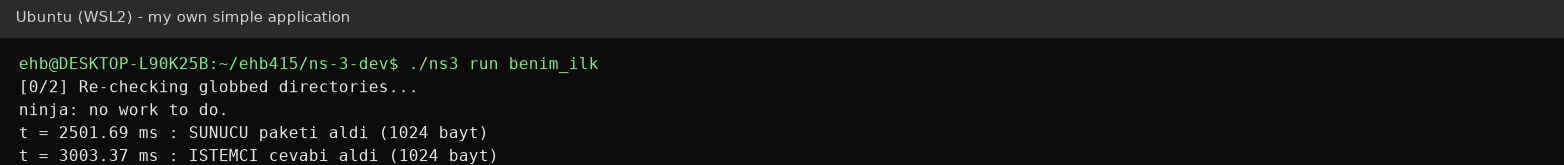
\includegraphics[width=\textwidth]{img/ns3_rapor_ilk.png}
\caption{\texttt{./ns3 run benim\_ilk} çıktısı.}
\end{figure}
Elle hesap: paket başlıklarıyla 1054 bayt, $1054\times 8/5\,\text{Mbps}=1{,}69$\,ms, artı 500\,ms kablo gecikmesi $=501{,}69$\,ms. Sunucu paketi $2000+501{,}69=2501{,}69$\,ms'de aldı, cevap aynı yoldan dönünce istemci $3003{,}37$\,ms'de aldı. Simülasyon çıktısı elle hesapla birebir tuttu.

\subsection*{Değerlendirme ve sonraki adımlar}
ns-3.48 ve 5G-LENA v5.1 kuruldu, derlendi ve hem hazır 5G örneği hem kendi programım doğru sonuç üretti. Sınırlamalar: 5G-LENA'da hazır bir sensing modeli yok, bu yüzden ns-3 yalnızca haberleşme tarafının maliyetini ölçecek; sensing yükünü simülasyonda temsil etme yolu henüz seçilmedi. Sonraki adımlar:
\begin{itemize}
\item Kullanıcı sayısını (1, 2, 5, 10, 20) değiştirip toplam throughput ve gecikmeyi ölçmek.
\item 5G-LENA'daki zamanlayıcıları (\texttt{nr-mac-scheduler-*}) incelemek; varsayılan olan \texttt{NrMacSchedulerTdmaRR}'dir.
\item Bandı daraltarak sensing yükünü taklit eden deney ve bunun alternatifi olan ``sensing'i ayrı trafik akışı olarak ekleme'' yollarını karşılaştırmak.
\end{itemize}


\clearpage
\section*{3. Bölüm B: OCUDU}
{\sffamily\small Hazırlayan: \fatih\par}

\subsection*{Projedeki yeri ve araç seçimi}
OCUDU, srsRAN Project'in devamı olan ve Linux Foundation çatısı altında geliştirilen açık kaynaklı bir \textbf{gerçek 5G baz istasyonu (gNB) yazılımıdır}. ns-3 gibi bir model değil, gerçek protokol kodudur. Projemizde, sensing için ayrılan kaynağın (PRS) haberleşmeye maliyetini gerçek bir zamanlayıcı (scheduler) üzerinde ölçmek için kullanılacak; bu, ns-3 sonuçlarına güvenilirlik katar. Gerçek bir radyo (USRP) gerekmeden çalışabilmesi için ZeroMQ (sanal RF) ve \texttt{testmode} özellikleri kullanıldı.

\subsection*{Kurulum}
\begin{center}\sffamily\small
\begin{tabular}{@{}ll@{}}
\toprule
Ortam & Windows 11 üzerinde WSL2, Ubuntu 24.04.5 LTS \\
Derleyici ve araçlar & Clang 18.1.3, CMake 3.28.3, ccache \\
Yazılım sürümü & OCUDU \texttt{release\_26\_10}, 26.10.0 (commit e0db566) \\
Seçenekler & \texttt{ENABLE\_ZEROMQ=ON}, \texttt{ENABLE\_EXPORT=ON}; yalnızca \texttt{gnb} hedefi \\
Süre ve disk & yaklaşık 23 dakika (\texttt{-j4}), yaklaşık 0,6 GB \\
\bottomrule
\end{tabular}
\end{center}
Resmi kurulum sayfası gcc 15.2 veya üstünü ya da Clang 14 ve üstünü önerir. Ubuntu 24.04'te gcc 13.3 olduğu için \textbf{Clang 18} kullandık. Komutlar (ayrıntı: \texttt{kurulum/05-ocudu.md}):
\begin{lstlisting}
sudo apt-get update
sudo apt-get install -y cmake make gcc g++ clang pkg-config \
    libmbedtls-dev libsctp-dev libyaml-cpp-dev libgtest-dev \
    libfftw3-dev libeigen3-dev libzmq3-dev ccache
mkdir -p ~/ehb415 && cd ~/ehb415
git clone --depth 1 --branch release_26_10 https://gitlab.com/ocudu/ocudu.git
cd ocudu && mkdir -p build && cd build
CC=clang CXX=clang++ cmake ../ -DENABLE_EXPORT=ON -DENABLE_ZEROMQ=ON \
    -DCMAKE_C_COMPILER_LAUNCHER=ccache -DCMAKE_CXX_COMPILER_LAUNCHER=ccache
make -j4 gnb
\end{lstlisting}
CMake çıktısında \texttt{The CXX compiler identification is Clang 18.1.3} ve \texttt{Found libZEROMQ} satırları görünmelidir.

\subsection*{Karşılaşılan sorunlar ve çözümleri}
\begingroup\sffamily\small
\begin{xltabular}{\textwidth}{@{}p{4.3cm}X@{}}
\toprule
\textbf{Sorun} & \textbf{Neden ve çözüm} \\
\midrule
CMake çıktısında \texttt{Found libZEROMQ} yok & ZeroMQ yalnızca yapılandırma sırasında algılanır. \texttt{libzmq3-dev} kurulup \texttt{build} klasörü silindi ve \texttt{cmake} yeniden çalıştırıldı. \\
Derleme çıktısında ``error'' kelimesi & Dosya adlarında geçiyor (\texttt{..\_error\_handler\_impl.cpp}). Gerçek hata \texttt{error:} ile ve dosya:satır bilgisiyle başlar. \\
\texttt{256QAM MCS table cannot be used for PDSCH with fallback DCI format} & İlk testmode denemesinde \texttt{pdsch/pusch mcs\_table: qam64} ayarı eksikti. Yapılandırma dosyasına eklenince hücre açıldı. \\
\texttt{Scheduling priority of thread ... not changed. Not enough privileges} & Gerçek zamanlı öncelik için \texttt{sudo} gerekir. WSL'de zararsızdır, hücrenin açılmasını engellemedi. \\
Günlükte \texttt{Real-time failure in RU: received late DL request} & WSL2 çekirdeği gerçek zamanlı olmadığı için beklenen bir uyarıdır. \\
Ölçüm tablosu görünmüyor & Tablo yalnızca etkileşimli terminalde (TTY) görünür. Program çalışırken \texttt{t} yazıp Enter'a basmak gerekir. \\
\bottomrule
\end{xltabular}
\endgroup

\subsection*{Örnek çalıştırma}
Kurulumu doğrulamak için gNB'yi radyo ve çekirdek ağ olmadan çalıştırdım (\texttt{ru\_dummy}, \texttt{no\_core}, 1 sanal kullanıcı; yapılandırma: \texttt{ocudu\_testmode.yml}). Program başladıktan sonra \texttt{t} yazıp Enter'a basarak canlı ölçüm tablosunu açtım.
\begin{lstlisting}
cd ~/ehb415/ocudu/build/apps/gnb
./gnb --version
./gnb -c ~/ehb415/ocudu_testmode.yml
\end{lstlisting}
\begin{figure}[h!]
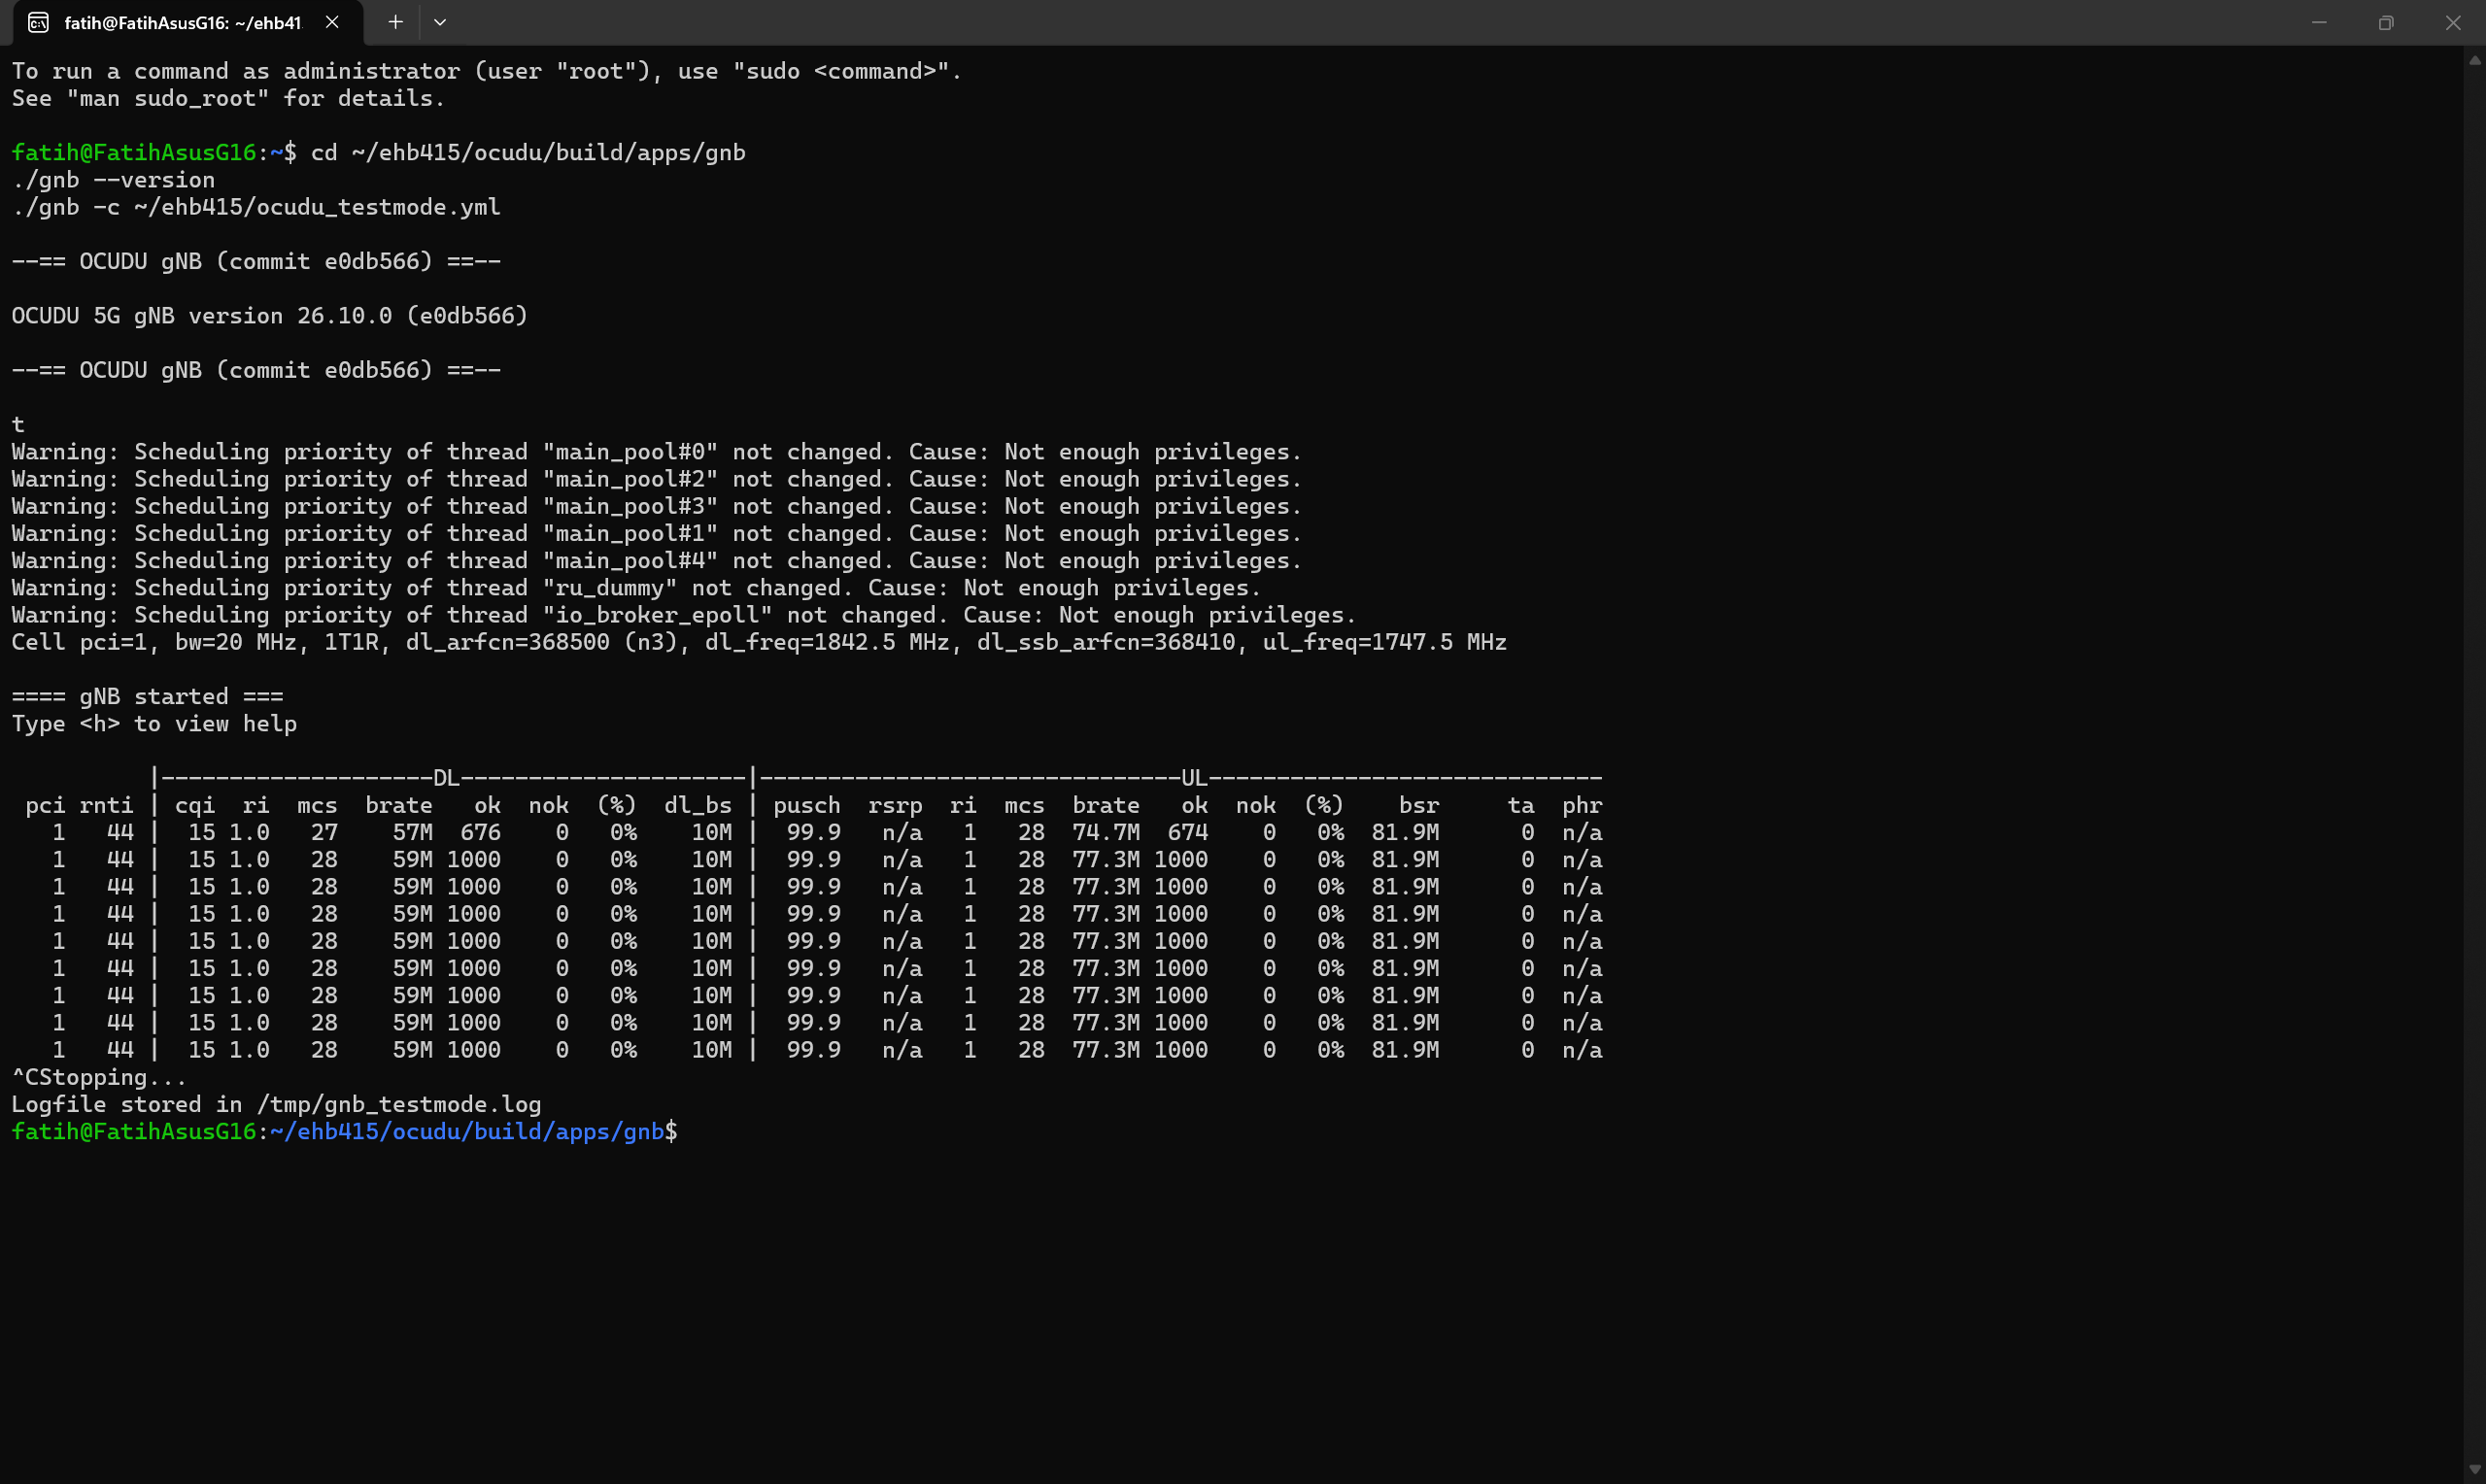
\includegraphics[width=\textwidth]{img/ocudu_terminal.png}
\caption{\texttt{gnb --version}, hücrenin açılması ve canlı ölçüm tablosu (WSL2 Ubuntu).}
\end{figure}
Çıktıda 26.10.0 (e0db566) sürümü ve n3 bandında 20\,MHz, 1T1R bir hücrenin açıldığı görülüyor. Tablonun kararlı satırlarında \textbf{DL hızı yaklaşık 59 Mbps, UL hızı 77,3 Mbps} ve her iki yönde başarılı blok sayısı \textbf{1000 blok/s} okundu. Ctrl+C'den sonra program \texttt{Stopping} mesajıyla düzgün kapandı. Bu çıktılar OCUDU'nun radyosuz test ortamında çalıştığını ve ölçüm üretebildiğini gösteriyor.

\subsection*{Değerlendirme ve sonraki adımlar}
OCUDU 26.10.0 derlendi ve testmode'da çalıştı. Sınırlamalar: (i) srsUE ve Open5GS ile uçtan uca test \textbf{yapılmadı}; resmi dokümandan aktarıldı, bu kurulumda çalıştırılmadı. (ii) WSL2 gerçek zamanlı olmadığından gerçek radyo (USRP) bağlantısı desteklenmiyor; bu proje için gerekmiyor. Sonraki adımlar:
\begin{itemize}
\item PRS (konumlama referans sinyali) periyodunu değiştirip DL hızındaki düşüşü ölçmek (PRS yokken 59,0 Mbps).
\item Birden fazla sanal kullanıcıyla aynı deneyi tekrarlamak.
\item Açık soru: 4 sembollük PRS neden 12 sembollük PRS ile aynı kaybı veriyor? Zamanlayıcı kodunda (\texttt{intra\_slice\_scheduler.cpp}) PDSCH için hangi sembol aralığına bakıldığı incelenecek.
\end{itemize}


\clearpage
\section*{4. Bölüm C: Sionna ve Sionna RT}
{\sffamily\small Hazırlayan: \nihat\par}

\subsection*{Projedeki yeri ve araç seçimi}
Sionna, NVIDIA'nın açık kaynaklı bağlantı düzeyi (link-level) simülatör kütüphanesidir; \textbf{Sionna RT} ise ışın izleme (ray tracing) ile gerçek bir şehir sahnesinde kanalı hesaplar. Projede Sionna \textbf{kazanç tarafını} ölçer: sensing'e ayrılan kaynak payı $\alpha$ arttıkça bir İHA'yı hangi mesafeden, ne olasılıkla ve ne doğrulukla bulabiliyoruz? Sionna RT, binaların görüş hattını kestiği gerçekçi bir senaryo (Münih sahnesi, 4,9\,GHz) sağlıyor. ns-3 ve OCUDU yalnızca bedeli ölçtüğü için, kazanç ölçülmeden ödünleşim (trade-off) çıkmaz.

\subsection*{Kurulum}
Kurulum iki ortamda yapıldı ve ikisinde de aynı paket sürümleri elde edildi.
\begin{center}\sffamily\small
\begin{tabular}{@{}lll@{}}
\toprule
 & \textbf{Ortam A: Ubuntu} & \textbf{Ortam B: Windows} \\
\midrule
İşletim sistemi & Ubuntu 22.04.5 LTS & Windows 11 \\
Python & sistem Python'u 3.10.12 & 3.11.9 (sanal ortam) \\
LLVM (Sionna RT için) & \texttt{libllvm14} (apt) & LLVM 23.1.3 (\texttt{winget}) \\
Sionna / sionna-rt & 1.2.2 / 1.2.2 & 1.2.2 / 1.2.2 \\
TensorFlow, Mitsuba, Dr.Jit & 2.21.0, 3.8.0, 1.3.1 & 2.21.0, 3.8.0, 1.3.1 \\
Süre ve disk & $\approx$5 dk (hızlı ağda), 2,8 GB & 15--30 dk, 2,1 GB \\
\bottomrule
\end{tabular}
\end{center}
\textbf{Ortam A (Ubuntu) komutları} (ayrıntı: \texttt{kurulum/03-sionna-ubuntu.md}):
\begin{lstlisting}
sudo apt update
sudo apt install -y python3-venv libllvm14 libatomic1
mkdir -p ~/venvs && python3 -m venv ~/venvs/ehb415
~/venvs/ehb415/bin/python -m pip install --upgrade pip
~/venvs/ehb415/bin/python -m pip install --retries 10 --timeout 60 "sionna==1.2.2" jupyterlab matplotlib scipy
\end{lstlisting}
\textbf{Ortam B (Windows) komutları} (PowerShell; ayrıntı: \texttt{kurulum/03-sionna-windows.md}). LLVM kurulumu \emph{yönetici} PowerShell ister:
\begin{lstlisting}
python -m venv C:\Users\$env:USERNAME\venvs\ehb415
C:\Users\$env:USERNAME\venvs\ehb415\Scripts\python.exe -m pip install --retries 10 --timeout 60 "sionna==1.2.2" jupyterlab matplotlib scipy
.\kur-llvm.ps1      # yonetici PowerShell: LLVM kurar ve DRJIT_LIBLLVM_PATH ayarlar
\end{lstlisting}
\texttt{sionna==1.2.2} sürümünü sabitlemek önemli: Python 3.11'de sürümsüz \texttt{pip install sionna} Sionna 2.2.0'ı seçer ve bizim betiklerimiz 1.2.2 içindir.

\subsection*{Karşılaşılan sorunlar ve çözümleri}
\begingroup\sffamily\small
\begin{xltabular}{\textwidth}{@{}p{4.4cm}X@{}}
\toprule
\textbf{Sorun} & \textbf{Neden ve çözüm} \\
\midrule
\texttt{ensurepip is not available} (Ubuntu) & \texttt{python3-venv} paketi yok. \texttt{sudo apt install -y python3-venv}. \\
\texttt{Could not import the Dr.Jit binary extension ... incompatible with the current interpreter} (Ubuntu) & Mesaj yanıltıcı: asıl neden Python sürümü değil, \texttt{libatomic.so.1} eksikliği. \texttt{sudo apt install -y libatomic1}. \\
\texttt{LLVM shared library ("libLLVM.so") could not be found} (Ubuntu) & \texttt{sudo apt install -y libllvm14}. \\
\texttt{LLVM-C.dll could not be found} (Windows) & LLVM kurulu değil ya da \texttt{DRJIT\_LIBLLVM\_PATH} ayarsız. \texttt{kur-llvm.ps1} (yönetici) çalıştırılır ve \textbf{yeni bir PowerShell} açılır (ortam değişkeni eski pencerelere yansımaz). \\
Sonda \texttt{free(): invalid pointer} veya \texttt{Segmentation fault} (Ubuntu) & TensorFlow, \texttt{sionna.rt}'den önce içe aktarılmış. \texttt{import sionna.rt} her zaman \textbf{ilk} satır olmalı. Windows'ta bu sorun yok. \\
Python 3.11'de beklenmedik Sionna 2.2.0 kurulumu & Sürüm sabitlenmemişti. \texttt{"sionna==1.2.2"} yazılır. \\
\texttt{TypeError: PathSolver ... 'samples\_per\_tx'} & Sionna 1.2.2'de parametre adı \texttt{samples\_per\_src}'dir; eski örnek kodlarda farklı geçer. \\
\texttt{TensorFlow GPU support is not available on native Windows} & Beklenen ve zararsız uyarı; Sionna CPU'da çalışır. \\
\bottomrule
\end{xltabular}
\endgroup

\subsection*{Örnek çalıştırma}
\subsubsection*{Kurulum doğrulaması (Ortam B, Windows)}
Önce paket sürümlerini listeledim, ardından iki doğrulama betiğini çalıştırdım: \texttt{sionna\_dogrulama.py} saf NumPy ile tek hedefli bir OFDM radar testi yapar ve Sionna'nın \texttt{ResourceGrid} nesnesini oluşturur; \texttt{sionna\_rt\_dogrulama.py} ise Münih sahnesini yükleyip ışın yollarını hesaplar.
\begin{figure}[h!]
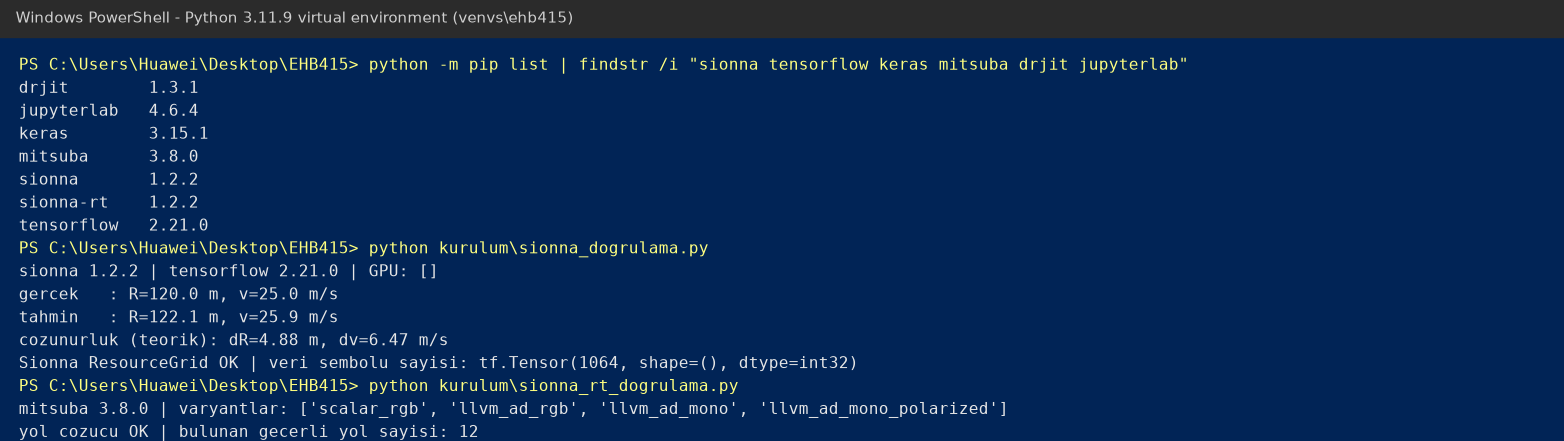
\includegraphics[width=\textwidth]{img/sionna_windows_terminal.png}
\caption{Paket sürümleri ve iki doğrulama betiğinin çıktısı (Windows PowerShell).}
\end{figure}
Radar testinde gerçek hedef 120,0\,m ve 25,0\,m/s iken tahmin 122,1\,m ve 25,9\,m/s çıktı; hatalar teorik çözünürlük hücresinin (4,88\,m ve 6,47\,m/s) içinde olduğundan sonuç doğrudur. Sionna RT 12 geçerli ışın yolu buldu.

\subsubsection*{Proje betikleri (Ortam A, Ubuntu)}
Ubuntu ortamında projenin iki betiğini çalıştırdım: \texttt{radar\_takip.py}, sembollerin $\alpha$ kadarını sensing'e ayıran basit bir radar modeliyle farklı mesafelerdeki bir İHA'yı tespit ediyor; \texttt{rt\_sehir.py} ise Sionna RT ile şehir sahnesinde radyo haritasını ve ışın yollarını hesaplıyor.
\begin{figure}[h!]
\centering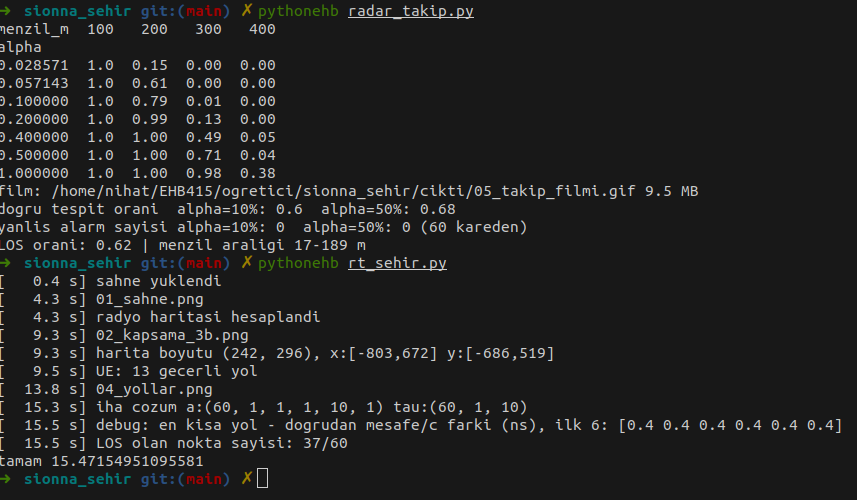
\includegraphics[width=0.78\textwidth]{img/sionna_ubuntu_terminal.png}
\caption{\texttt{radar\_takip.py} tespit olasılığı tablosu ve \texttt{rt\_sehir.py} çıktısı (Ubuntu).}
\end{figure}
\begin{itemize}
\item \textbf{Tespit olasılığı:} 100\,m'de $\alpha$ ne olursa olsun İHA bulunuyor. 200\,m'de $\alpha=\%2{,}9$ için 0,15, $\alpha=\%20$ için 0,99. 300\,m'de ancak $\alpha=\%100$'de 0,98; 400\,m'de en fazla 0,38.
\item \textbf{Takip senaryosu (60 kare):} doğru tespit oranı $\alpha=\%10$ için 0,60, $\alpha=\%50$ için 0,68; yanlış alarm yok.
\item \textbf{Görüş hattı:} 60 noktanın 37'sinde (\%62) İHA ile verici arasında doğrudan görüş var. Tespit oranlarının bu orana yakın çıkması, tespitin büyük ölçüde doğrudan görüş olan karelerden geldiğini düşündürüyor.
\item \textbf{Sionna RT süresi:} sahne 0,4\,s'de yüklendi, tüm adımlar yaklaşık 15,5\,s'de bitti.
\end{itemize}
\begin{figure}[h!]
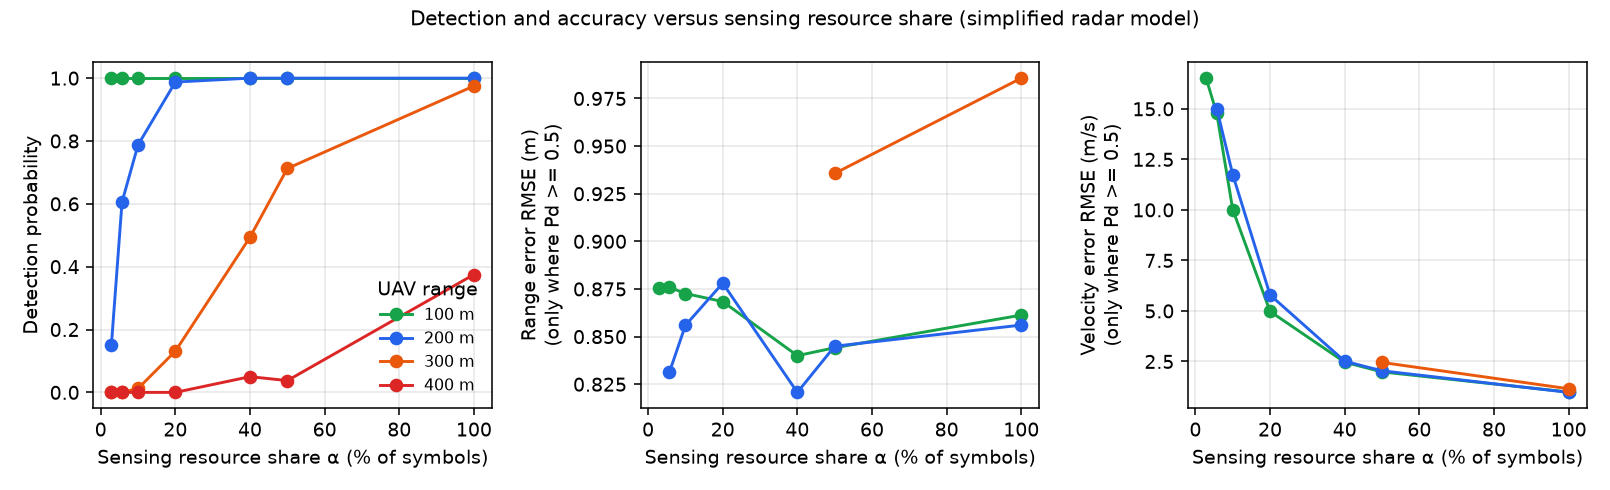
\includegraphics[width=\textwidth]{img/sionna_grafik.png}
\caption{Sensing payı $\alpha$ arttıkça tespit olasılığı, menzil hatası ve hız hatası.}
\end{figure}
Grafikte menzil hatası $\alpha$'dan neredeyse bağımsız ($\approx$0,8--1,0\,m); hız hatası ise $\alpha$ arttıkça 15--16\,m/s'den yaklaşık 1\,m/s'ye düşüyor. Menzil çözünürlüğü sembol sayısına değil bant genişliğine bağlı olduğu için menzil doğruluğu pek değişmiyor; sensing'e daha çok sembol ayırmak özellikle hız (Doppler) kestirimini iyileştiriyor.
\begin{figure}[h!]
\centering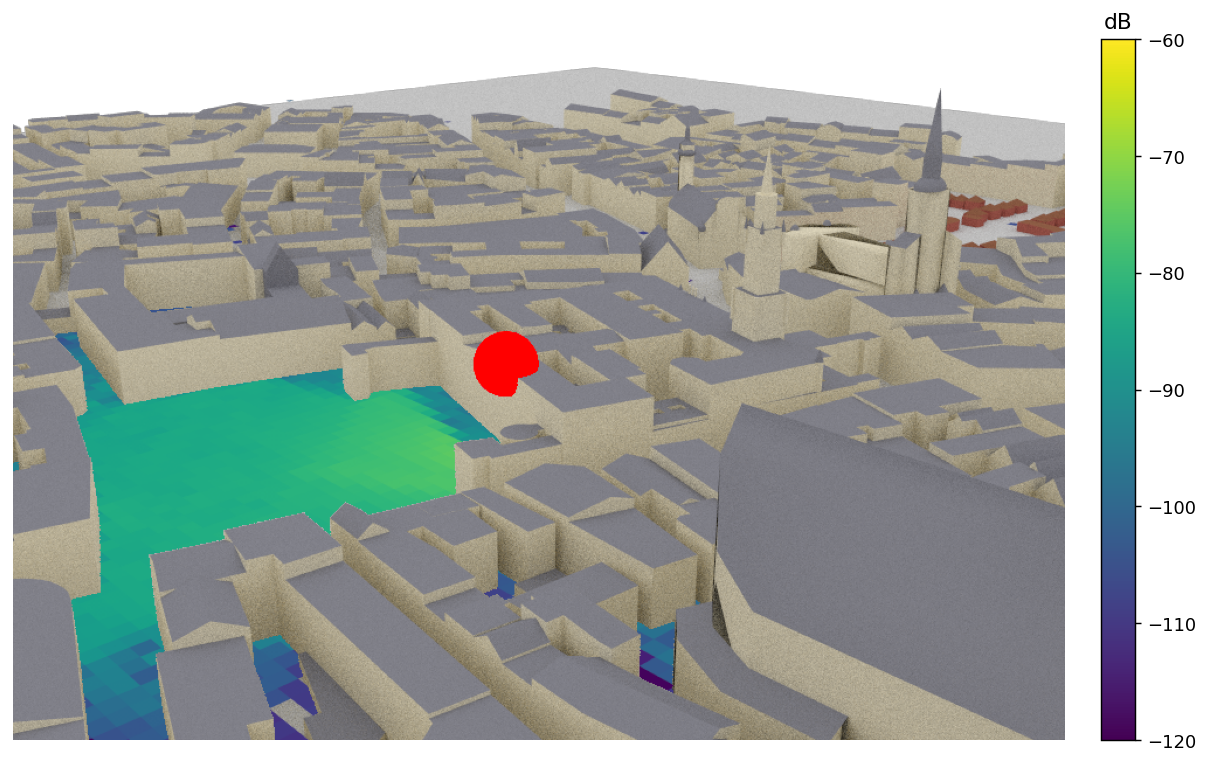
\includegraphics[width=0.62\textwidth]{img/sionna_kapsama3b.png}
\caption{Sionna RT ile hesaplanan radyo haritası (yol kazancı, dB). Kırmızı küre vericinin (gNB) konumu; binaların arkasında sinyal belirgin biçimde zayıflıyor.}
\end{figure}

\subsection*{Değerlendirme ve sonraki adımlar}
Sionna 1.2.2 ve Sionna RT iki farklı ortamda (Ubuntu 22.04 ve Windows 11) kuruldu, doğrulama betikleri hatasız bitti ve proje betikleri beklenen sonuçları üretti. Sınırlamalar: GPU kullanılmadı (CPU); radar modeli basitleştirilmiş bir modeldir (``oyuncak radar''), tam bir 3GPP kanal modeli değildir. Sionna RT çıktısını ns-3'e besleyen SioLENA modülü \textbf{denenmedi}. Sonraki adımlar:
\begin{itemize}
\item Radar kodundaki \texttt{radar()} fonksiyonunu (2B FFT ile menzil ve hız kestirimi) satır satır incelemek.
\item Artık öz-girişim (\texttt{X\_SI\_DB}) değerini değiştirip tespit olasılığına etkisini ölçmek.
\item Elde edilen $P_d$ ve hata eğrilerini TR~38.765'in hedefleriyle ($P_{md}\le\%5$) karşılaştırmak.
\end{itemize}


\section*{5. Genel değerlendirme}
Üç araç da kuruldu ve doğrulama çıktıları beklenen sonuçları verdi. Araçlar birbirini tamamlıyor: Sionna algılamanın \emph{kazancını}, ns-3 ve OCUDU ise haberleşmenin \emph{bedelini} ölçer. Önceden bilinen sınırlamalar: 5G-LENA'da hazır bir sensing modeli yok (sensing yükünü ns-3'te nasıl temsil edeceğimiz seçilecek); OCUDU'da uçtan uca (srsUE + Open5GS) test yapılmadı; Sionna'da GPU kullanılmadı ve radar modeli basitleştirilmiştir; Sionna RT'nin ns-3'e bağlanması (SioLENA) denenmedi.

\begingroup\sffamily\small
\begin{xltabular}{\textwidth}{@{}p{3.6cm}X@{}}
\toprule
\textbf{Sorumlu} & \textbf{Sonraki aşamadaki iş} \\
\midrule
\taha & 3GPP TR 38.765'in incelenmesi, metrik sözlüğü, $\alpha$ tanımının üç araçta ortaklaştırılması, rapor \\
\aziz & ns-3'te kullanıcı sayısı ve bant taraması, zamanlayıcı karşılaştırması, sensing yükünün temsil yolunun seçimi \\
\fatih & OCUDU'da PRS periyodu ve çok kullanıcılı deneyler; PRS'in PDSCH'e etkisinin zamanlayıcı kodunda incelenmesi \\
\nihat & Radar modelinin incelenmesi, tespit olasılığı ve hata eğrilerinin 3GPP hedefleriyle karşılaştırılması \\
\bottomrule
\end{xltabular}
\endgroup
\end{document}
